%article using font-size 12 and A4-size
\documentclass[a4paper,12pt]{article}

%use danish hyphenation and titles
%handle utf8-characters
\usepackage[danish]{babel}
\usepackage[utf8]{inputenc}
\usepackage[T1]{fontenc}

%for images
\usepackage[pdftex]{graphicx}

%allow nested figures
\usepackage{subfigure}

%control line spacing
\usepackage{setspace}
%\singlespacing
\onehalfspacing
%\doublespacing

%set margins
%\usepackage[margin=0.75in]{geometry}

%allows margin-notes
%good for work in progress papers
%\usepackage{marginnote}

%allows pretty quoting using ``'' or `'
\usepackage{upquote}

%two definitions of the color grey
\usepackage{color}
\definecolor{listinggray}{gray}{0.9}
%\definecolor{lbcolor}{rgb}{0.9,0.9,0.9}

%allows pretty source code
\usepackage{listings}
\lstset{
	language=,
	literate=
		{æ}{{\ae}}1
		{‚àö‚àè}{{\o}}1
		{å}{{\aa}}1
		{‚àö√ú}{{\AE}}1
		{√ò}{{\O}}1
		{√Ö}{{\AA}}1,
	backgroundcolor=\color{listinggray},
	tabsize=3,
	rulecolor=,
	basicstyle=\scriptsize,
	upquote=true,
	aboveskip={1.5\baselineskip},
	columns=fixed,
	showstringspaces=false,
	extendedchars=true,
	breaklines=true,
	prebreak =\raisebox{0ex}[0ex][0ex]{\ensuremath{\hookleftarrow}},
	frame=single,
	showtabs=false,
	showspaces=false,
	showstringspaces=false,
	identifierstyle=\ttfamily,
	keywordstyle=\color[rgb]{0,0,1},
	commentstyle=\color[rgb]{0.133,0.545,0.133},
	stringstyle=\color[rgb]{0.627,0.126,0.941},
}
%captions on listings
\usepackage[center,font=small,labelfont=bf,textfont=it]{caption}

%allows fancy enumeration
\usepackage{enumerate}

%allows use of the BibTex for the bibliography
\usepackage[numbers]{natbib}

%make references and URLs in the pdf to clickable links
\usepackage{hyperref}

%proper header formatting
\usepackage{fancyhdr}
\pagestyle{fancy}
\lhead[]{} %clear standard settings
\chead[]{} %clear standard settings
\rhead[]{\rightmark} %current section
\lfoot[]{} %clear standard settings
\cfoot[]{\thepage} %current page number 
\rfoot[]{} %clear standard settings

%define paper title, author and date
%if date is empty, defaults to current date
\title{Kontekstuel analyse}
\author{Yaser Hashimi og Julie Engholm}
\date{Oktober 9th - 2013}

\begin{document}
\maketitle %insert the defined title
\newpage
\tableofcontents %generate table of content
\newpage

\clearpage %clears float-buffer - inserting those missing - and starts new page

\section{PACT analyse}
\subsection{People}
Disse brugere vil man kunne forvente vil bruge låsesystemet.

\begin{itemize}
    \item Voksne der er husejere
    \item Børn til husejere
    \item Personer der er åben for ny teknologi
    \item Personer der er erfarne it-brugere.
    \item Typer, der gerne vil holde øje med deres hjem.
\end{itemize}

\subsection{Activities}
Dette er opgaverne man vil kunne udføre ved låsesystemet.

\begin{itemize}
    \item Låse op og i
    \item Aflæse om låsen er åben eller låst
    \item Give en midlertidig nøgle
    \item Gøre en nøgle ugyldig, så den ikke kan bruges til låsen
    \item Se en log over interaktioner med låsen på en bestemt dato
    \item Ændre brugerprivilegier eks. lade en bruger uddele nøgler eller se en log over interaktioner med låsen på en bestemt dato
    \item Se hvem der har nøgle til låsen
\end{itemize}


\subsection{Context}
Dette er situationer brugere muligvis vil bruge låsesystemet.

\begin{itemize}
    \item En person skal lukke en håndværker ind til reparationsarbejde mens han
ikke er hjemme.
    \item Når du får et opkald fra en i familien som har glemt sin nøgle og vil ind.
    \item En person er taget på arbejde og kan ikke huske om vedkommende låste døren.
    \item Brugeren vil finde ud af hvem der har brugt låsen den forrige dag.
    \item Brugeren vil fratage en lejers digitale nøgle.
    \item Hvis du fysisk ikke kan bevæge dig hen til døren.
\end{itemize}

\subsection{Technology}
Application vil blive kørt på en smartphone, tablet eller datamat med adgang til internettet.



\section{Fremgangsmåde}

En række interviews er i forbindelse med denne opgave blevet gennemført. Interviewenes formål
var at belyse brugeres forventninger til et digitalt låsesystem. Ud fra disse fundne
forventninger er der opstillet en række anbefalinger til ændringer i features, indhold og
organisering. Som en del af interviewet blev der udført kort gennemgang af en prototype. Dette
hjalp til at konkretisere brugerens forventninger.
\\ \\
Prototypen blev lavet på papir i hånden.

\subsection{Anvendt metode}

Hvert interview startede med at undersøge aspekter brugerens baggrund relateret til denne opgave:
computererfaringer, interneterfaringer, webhandelserfaringer og erfaringer med forskellige låsesystemer samt generelt internetstyrede løsninger til hjemmet.
\\ \\
Herefter blev spørgsmål stillet til brugerens forventninger til et digitalt låsesystem.
I selve interviewet blev der udført en gennemgang af en prototype vi havde udviklet, hvor brugerne fik lov at udforkse mulighederne, med nogle små opgaver.
Opgaverne afspejlede de grundlæggende arbejdsopgaver for hjemmesiden ("core tasks"). Undervejse noteredes komentarer til konkrete funktioner.
\\ \\
Efter testen blev deltagerne debriefet, og eventuelle kommentarer til prototypen blev tilføjet, og enkelte spørgsmål blev reevalueret.
\\ \\
Som evaluering undervejs i forløbet blev der efter hvert interview i gruppen diskuteret, om alt
kom med, hvilke resultater der var opnået, og eventuelt hvad der skulle laves af ændringer til
næste interview. Efter alle fem interviews var gennemført blev de samlede resultater og erfaringer
diskuteret i gruppen inden rapporten blev påbegyndt.


\subsection{Diskussion af metoden}

Interviewene er gennemført ud fra en tjekliste (se appendix A) og der er under interviewet brugt
åbne spørgsmål der følger master-apprentice paradigmet. Dette lægger op til den interviewedes
egne erfaringer og tanker, som anbefalet i kursuslitteraturen.


\subsection{Interviewdeltagere}

Der er tre kvinder og to mænd i gruppen af testdeltagere. Alle deltagerne kunne potentielt i
realiteten være kunder til et digitalt låsesystem. Ingen af deltagerne arbejder med IT som
hovedprofession.
\\  \\
\begin{tabular}{|l|l|l|l|l|l|}
	\hline Deltager & Køn & Alder & Profession & Postnummer & Interneterfaring \\
	\hline 1 & K & 23  & Stud. Global studies, RUC & 2300 & Erfaren \\
	\hline 2 & M & 26 & Stud. Matematik, KU & 2605 & Erfaren\\
	\hline 3 & K & 25 & Stud. Fysik, KU & 2200 & Erfaren \\
	\hline 4 & M & 25 & Stud. Biologi, KU & 2300 & Meget erfaren \\
	\hline 5 & K & 19 & Stud. HF, Frederiksberg & 2605 & Lidt erfaren \\
	\hline
\end{tabular}
\\ \\

Interneterfaring er klassificeret af testpersonen i henhold til disse grupperinger:
\begin{itemize}


\item Intet (Har aldrig hørt om det, eller kun læst om det 
\item Tilskuer (Har set andre personer bruge internettet)  
\item Begynder (Har brugt én eller to gange)
\item Lidt erfaren (Bruger det regelmæssigt)
\item Erfaren (Bruger søgefaciliteter uden problemer)
\item Meget erfaren (Har udviklet hjemmesider, kender til HTML)

\end{itemize}

\section{Interviewresultater}
Citater fra testdeltagere står i citationstegn. "Dette er altså et eksempel på et testdeltagercitat".
\subsection{Erfaringer med og brug af traditionelle fysiske låse}

To testdeltagere (1 og 3)bruger deres nøglebundt mere end 25 gange om dagen, mens (2, 4 og 5) kun bruger det 5-10 gange om dagen.
\\ \\
To destdeltagere (1 og 3) siger at det føler sig "afhængige" af deres fysiske nøgle.
\\ \\
To testdeltagere (3 og 4) siger at de ikke altid har alle deres nøgler på sig, men supplerer deres nøglebundt specielle nøgler når de ved de skal bruge dem.
\\ \\
Ingen af testdeltagerne har mistet deres nøglebundt (permanent/langvarigt) mere end en gang.
\\ \\
Ingen af testdeltagerne har fået lavet en kopi af en fysisk nøgle mere end 3 gange i deres liv.
\\ \\
Alle testdeltagere sagde, at "få nøgler til mange steder" passede bedre end "mange nøgler til få steder" når de skulle beskrive deres nøglebundt.
\\ \\
En af testdeltagerne (3), har en enkelt nøgle, som af og til ligger derhjemme når hun skal bruge den, hvilket er et irritationsmoment.

\subsection{Erfaringer fra andre digitale låse}

3 af deltagerne (1,3 og 5), fortæller om et låsesystem på et kollegie, hvor et opkald på dørtelefonen på hoveddøren går til beboerens telefon, som så kan lukke besøgende ind, uanset hvor vedkommende er med sin telefon.
Alle deltagere der nævnte systemet, fandt det meget smart.
\\ \\
Alle testdeltagerne havde erfaring med at bruge chiplåse til døre.


\subsection{Erfaringer med andre internetstyrede løsninger}
Ingen af brugerne har internetstyrede løsninger til hjemmet. En enkelt (4), har dog en ven, som har bygget en digital lås til sin private dør.
\\ \\
To brugere (1 og 4) har set løsninger hvor man kunne afspille musik på afspillere i hjemmet styret med en internetkompatibelt stykke teknologi over netværket.
\\ \\
En enkelt bruger (3) bruger netbank på sin smartphone. 

\subsection{Generelle forventninger}

Alle deltagere forventer at det skal være ligeså nemt, eller nemmere, at låse døre op med smartphones som det er med en normal, fysisk nøgle.
\\ \\
En deltager (1), forventer at der er en sikkerhedsforanstaltning der sender en sms til telefonen hvis en fysisk lås forsøges "brudt op eller på anden vis kommpromitteret".

\subsection{Features, der ville være gode, men som ikke er forventet}
Deltager 1 nævner, at hun gerne vil have det implementeret på sit studie, så hun nemt kunne få adgang til fx. kontorer eller grupperum når der var behov, uden at skulle forbi receptionen.
\\ \\
To deltagere (1 og 4) nævner, at de gerne så at et digitalt låsesystem skulle være kompatibelt med andre sikkerhedssystemer som fx. overvågning og alarmsystemer.
\\ \\
Deltager 1 nævner, at hun gerne så en funktion der kunne vise de steder man havde adgang til gennem app'en på et kort, så man direkte kunne hente en rutevejledning til det pågældende sted, inde i app'en.


\subsection{Features og indhold der ville være dårligt}
3 testdeltagere (1, 2 og 3), nævner, at mere end de allermest basale funktioner (lås op/i, samt se status på lås), ikke har plads i app'ens primære forside, og at de ville være træt af et design med "mange flere funktioner, allerede på forsiden, end man kan overskue, for så kommer man aldrig igang" (citat fra 3).
\\ \\
En deltager (1), nævner at et fingeraftrykslås ville være ufyldestgørende som sikkerhedsforanstaltning.

\subsection{Holdninger til anvendelse}
Alle testdeltagere kunne se sig selv anvende systemet i deres private hjem i fremtidem såfremt sikkerheden var god nok. 
\\ \\
1 testdeltagerne (2) ville anvende det i sit private hjem nu.

\subsection{Tillid og sikkerhed}

Alle testdeltagere understreger at de har "meget høje krav" (citat fra 1), eller tilsvarende til sikkerheden.

To af testdeltagerne (1 og 4) beskriver deres syn på ny teknologi som "skeptisk", og ville ikke umiddelbart have tillid til låsesystemer implementeret på smartphones.

Ingen af testdeltagerne kan komme på en løsning som de både finder sikker og let nok. "Jo lettere det er at bruge, jo lettere er det jo for det meste at misbruge" (citat fra 4).

\subsection{Forventning vs. prototype}
Begge de første testdeltagere fandt funktionaliteten "Bestil fysisk nøgle" der optrådte i den første protoype, overflødig, da behovet meget sjældent opstår. \\"Jeg ville jo alligevel ringe til firmaet, så det er lidt spild af plads" (citat fra 1)
\\ \\
En testdeltager (2) fandt grovprototypens tekster var forvirrende men at selve systemet ellers virkede simpelt. Det kunne han godt lide.
\\ \\
To af testdeltagerne (3 og 4) mente at prototypen nogenlunde passede til deres forventninger til hvad de skulle se.
\\ \\
En af testdelagerne (1), var "positivt overrasket" over layoutet der var "intuitivt" og viste "det der skal bruges". \\ 
Desuden var hun ligeledes positivt overrasket over engangs- og tidsbegrænsningsmuligheden for uddelte nøgler. "Det er jo vildt smart, så skal man ikke tage fri fra arbejde for at få aflæst sin vandmåler i fem minutter"


\section{Kerneopgaver}
Dette er de grundlæggende arbejdsopgaver vi fandt ved brainstorm inden interviewsne.

\begin{itemize}
    \item Åbne og låse
    \item Se om lås er åbent eller låst
    \item Uddele nøglekopier til andre
    \item Gøre en nøgle ugyldig, så den ikke kan bruges til låsen
    \item Se en log over interaktioner med låsen på en bestemt dato
    \item Ændre brugerprivilegier eks. lade en bruger uddele nøgler
\end{itemize}
Følgende punkter er tilføjet på grundlag af interviewsne.

\begin{itemize}
    \item Give en midlertidig nøgle
    \item Se hvem der har nøgler til låse
\end{itemize}
Til sidst blev punktet at kunne bestille en fysisk nøgle via app'en fjernet da der fleste fandt dette unødvendigt.

\section{Målgruppebeskrivelser}
Følgende 4 bruger profiler er opnået gennem brainstorming og diskussion i gruppen.
\\
Primære brugergrupper:
\begin{itemize}
    \item Husejere
    \item Børn af husejere
    \item Personer der er åbne overfor ny teknologi
\end{itemize}
Sekundære brugergrupper er firmakunder som boligblokke, instutioner, firmaer osv. fokus ligger dog på private kunder jvf. oplæg.

\subsection{Uddybende beskrivelse af målgruppen personer der er åbne overfor ny teknologi}
Personer der er åbne overfor ny teknologi vil anvende låsesystemet mange gange om ugen. De bruger den primært til låse op og i, tjekke om alt er låst eller hvis de en sjældent gang får håndværker besøg at uddele nøgle.
\\ \\
Målgruppen er erfarne smartphone brugere. De forstår terminologien omkring låse.
\\ \\
Målgruppen bruger smartphones, men har ikke brugt en application til at åbne og låse med før fysiske låse før. De er erfarne brugere af internettet og de har alle adgang til dette hjemmefra.
\\ \\
Målgruppen kender opbygningen af generelle apps, da de bruger andre. De ved ikke hvordan smarthphonen eller applicationerne fungerer internt. Det virker bare.
\\ \\
Målgruppen vil gøre brug låsesystemet oftere end de andre målgrupper.

\section{Personas}
I det følgende er der opstillet to brugerkarakteristikker. Den første er i målgruppen \emph{personer der er åbne overfor ny teknologi}. Den anden er i målgruppen \emph{husejere}

\subsection{Handy Tom}
\begin{figure}[h!]
\centering

\includegraphics[scale=0.5]{tom}
\caption{Foto lånt af http://haandvaerkere.wordpress.com}
\label{fig: tom}
\end{figure}
Tom er 53 år og bor på Amager. Han arbejder som gårdmand for kommunen. Han har 2 børn og er gift.
\\ \\
Tom har haft sin smartphone i halvandet år nu. Han er forsigtig med sin telefon og plejer at få hjælp af sin svigersøn når han skal hente nye applicationer.
\\ \\
Når der er noget i hjemmet der skal fixes er det Tom som plejer at tage sig af dette. Han har hænderne skruet ordentligt på og dygtig til alt håndværk.
\\ \\
Tom bliver nok gange nød til at tage fri fra arbejde for at lukke håndværkere ind når han en sjældent gang ikke kan løse dette selv og har en reservenøgle liggende hos naboen til når datteren glemmer sin.

\subsection{Nørdede Niels}
\begin{figure}[h!]
\centering

\includegraphics[scale=0.8]{niels}
\caption{Foto lånt af http://www.computerworld.dk}
\label{fig: niels}
\end{figure}
Niels er 28 år, og bor på en andelslejelighed i Vanløse. Han har læst Matematik og Teknologi på DTU. Han har arbejdet på Oticon i et års tid.
\\ \\
Han bor sammen med sin kæreste, som kalder ham for sin nørd. Hun beskriver ham som, hjælpeløs uden sin smartphone. Han har alle mulige smarte applicationer.
\\ \\  
Niels har stor interesse for ny teknologi. Han kan godt lide at købe noget nyt på amazon og lege med dette. Det sidste han købte var en drone han kunne styre med sin smartphone.
\\ \\
Han syntes at det vil være nemmere at have sine nøgler digitalt, da de fysiske generer ham. Han har dog sine forbehold for sikkerheden.

\section{Scenarier}
\subsection{Toms brug af låsesystemet}
Det er tirsdag formiddag og Tom er på arbejde. Han har en aftale med håndværker der skal se på hvorfor der kun er koldt vand. Håndværkeren kan være det mellem 12:00-14:00. Han aftaler med håndværkeren at han får en nøgle som han kan bruge via en smartphone.
\\ \\
Senere på aftenen tjekker svigersønnen og Tom oversigten over hvornår håndværkeren havde været forbi og var gået igen.

\subsection{Niels brug af låsesystemet}
Det er tirsdag aften. Niels har en aftale om at mødes med en ven hjemme hos Niels og få et par drinks og tage i byen. Niels tager forbi supermarkedet for at købe ind til at lave drinks. Vennen ringer og siger at han står ude foran døren, men at ingen svarer. Niels åbner for låsen via sin smartphone og fortæller sin ven at han snart er hjemme.

\section{Erfaringer}
Vi har gjort os følgende erfaringer mht. interviewprocessen:
\begin{itemize}
    \item Vi har lært, at for en system af denne type, skulle vi have været bedre til at finde relevante interviewdeltagere, idet der kommer til at mangle repræsentanter for flere generationer i vores valg.
    \item Som interviewer skal man gøre sig meget umage ikke at komme til at stille ledende spørgsmål.
    \item Som interviewer skal man være meget nysgerrig for at bore dybt nok i de spørgsmål som man stiller, så at man rent faktisk får en dybere indsigt end den overfladiske.
    \item Som interviewer skal man være saglig og finder ud af hvad personen man interviewer mener og ikke skubbe sine egne meninger over på denne.
\end{itemize}


\newpage 
\appendix
\section{Tjekliste}
Følgende tjekliste bliver brugt som støtte i interviewene til at guide samtalen. \\
Disse punkter indleder interviewet og forklarer brugeren hvad der skal foregå og hvorfor:

\begin{itemize}
    \item Vi vil vise dig en tidlig udgave (prototype) af låsesystemet.
    \item Hvad er dine internet-færdigheder? Bruger du din smartphone ofte? Hvilke slags app bruger du?
\end{itemize}

Disse punkter sikrer at relevante emner omkring brugerens forventninger til låsesystemet bliver dækket i interviewene:

\begin{itemize}
    \item Hvor ofte bruger du en lås?
    \item Hvor mange nøgler er der i dit nøglebundt?
    \item Har du mange nøgler til få steder, eller få nøgler til mange steder?
    \item Bruger du i forvejen nogle internetstyrede løsninger i dit hjem (fx. lys, musikanlæg etc.)?
    \item Hvornår smed du sidst din nøgler væk?
    \item Hvornår skulle du sidst bruge en kopi af en nøgle?
    \item Har du brugt en digital lås før? (Evt. hotel el. lign.) ?
    \item Vil du betegne dig selv som en person der generelt har tillid til ny teknologi?
    \item Hvilke forskellige typer af nøgler kender du (kort, chip, fingeraftryk etc.)?
    \item Hvad syntes du om at kunne åbne og låse med din smartphone?
    \item Hvilke funktioner kunne låsesystemet have som du syntes var smart?
    \item Hvilke funktioner kunne låsesystemet have som du syntes var unødvendigt?
    \item Kunne du finde på at bruge låsesystemet?
\end{itemize}
Følgende punkter vil blive stillet efter demonstrationen af prototypen:

\begin{itemize}
    \item Hvordan lever låsesystemet op til dine forventninger?
    \item Syntes du der mangler noget?
    \item Kan du nævne to ting du kunne lide og to ting du ikke kunne lide ved låsesystemet?
    \item Ville du vælge en sådan løsning til dit eget hjem?
    \item Hvilke sider syntes du kunne blive forbedret?
    \item Hvorfor ville du eller ville du ikke bruge sådan et låsesystem i fremtiden?
    \item Ville du anvende dette låsesystem som supplement til fysiske nøgler, eller som din primære låsemetode?
\end{itemize}

\section{Prototype}

Herunder ses skærmbilleder fra vores prototype. Ved interviws er brugt udklippede kopier af de forskellige skærmbilleder og pop-ups/downs til at vise handlinger ved "klik på skærmen". Udganspunktet vises dog her, for overskuelighed skyld. Brugerne så ikke kommentarerne ved siden af skærmbillederne.
\\ \\
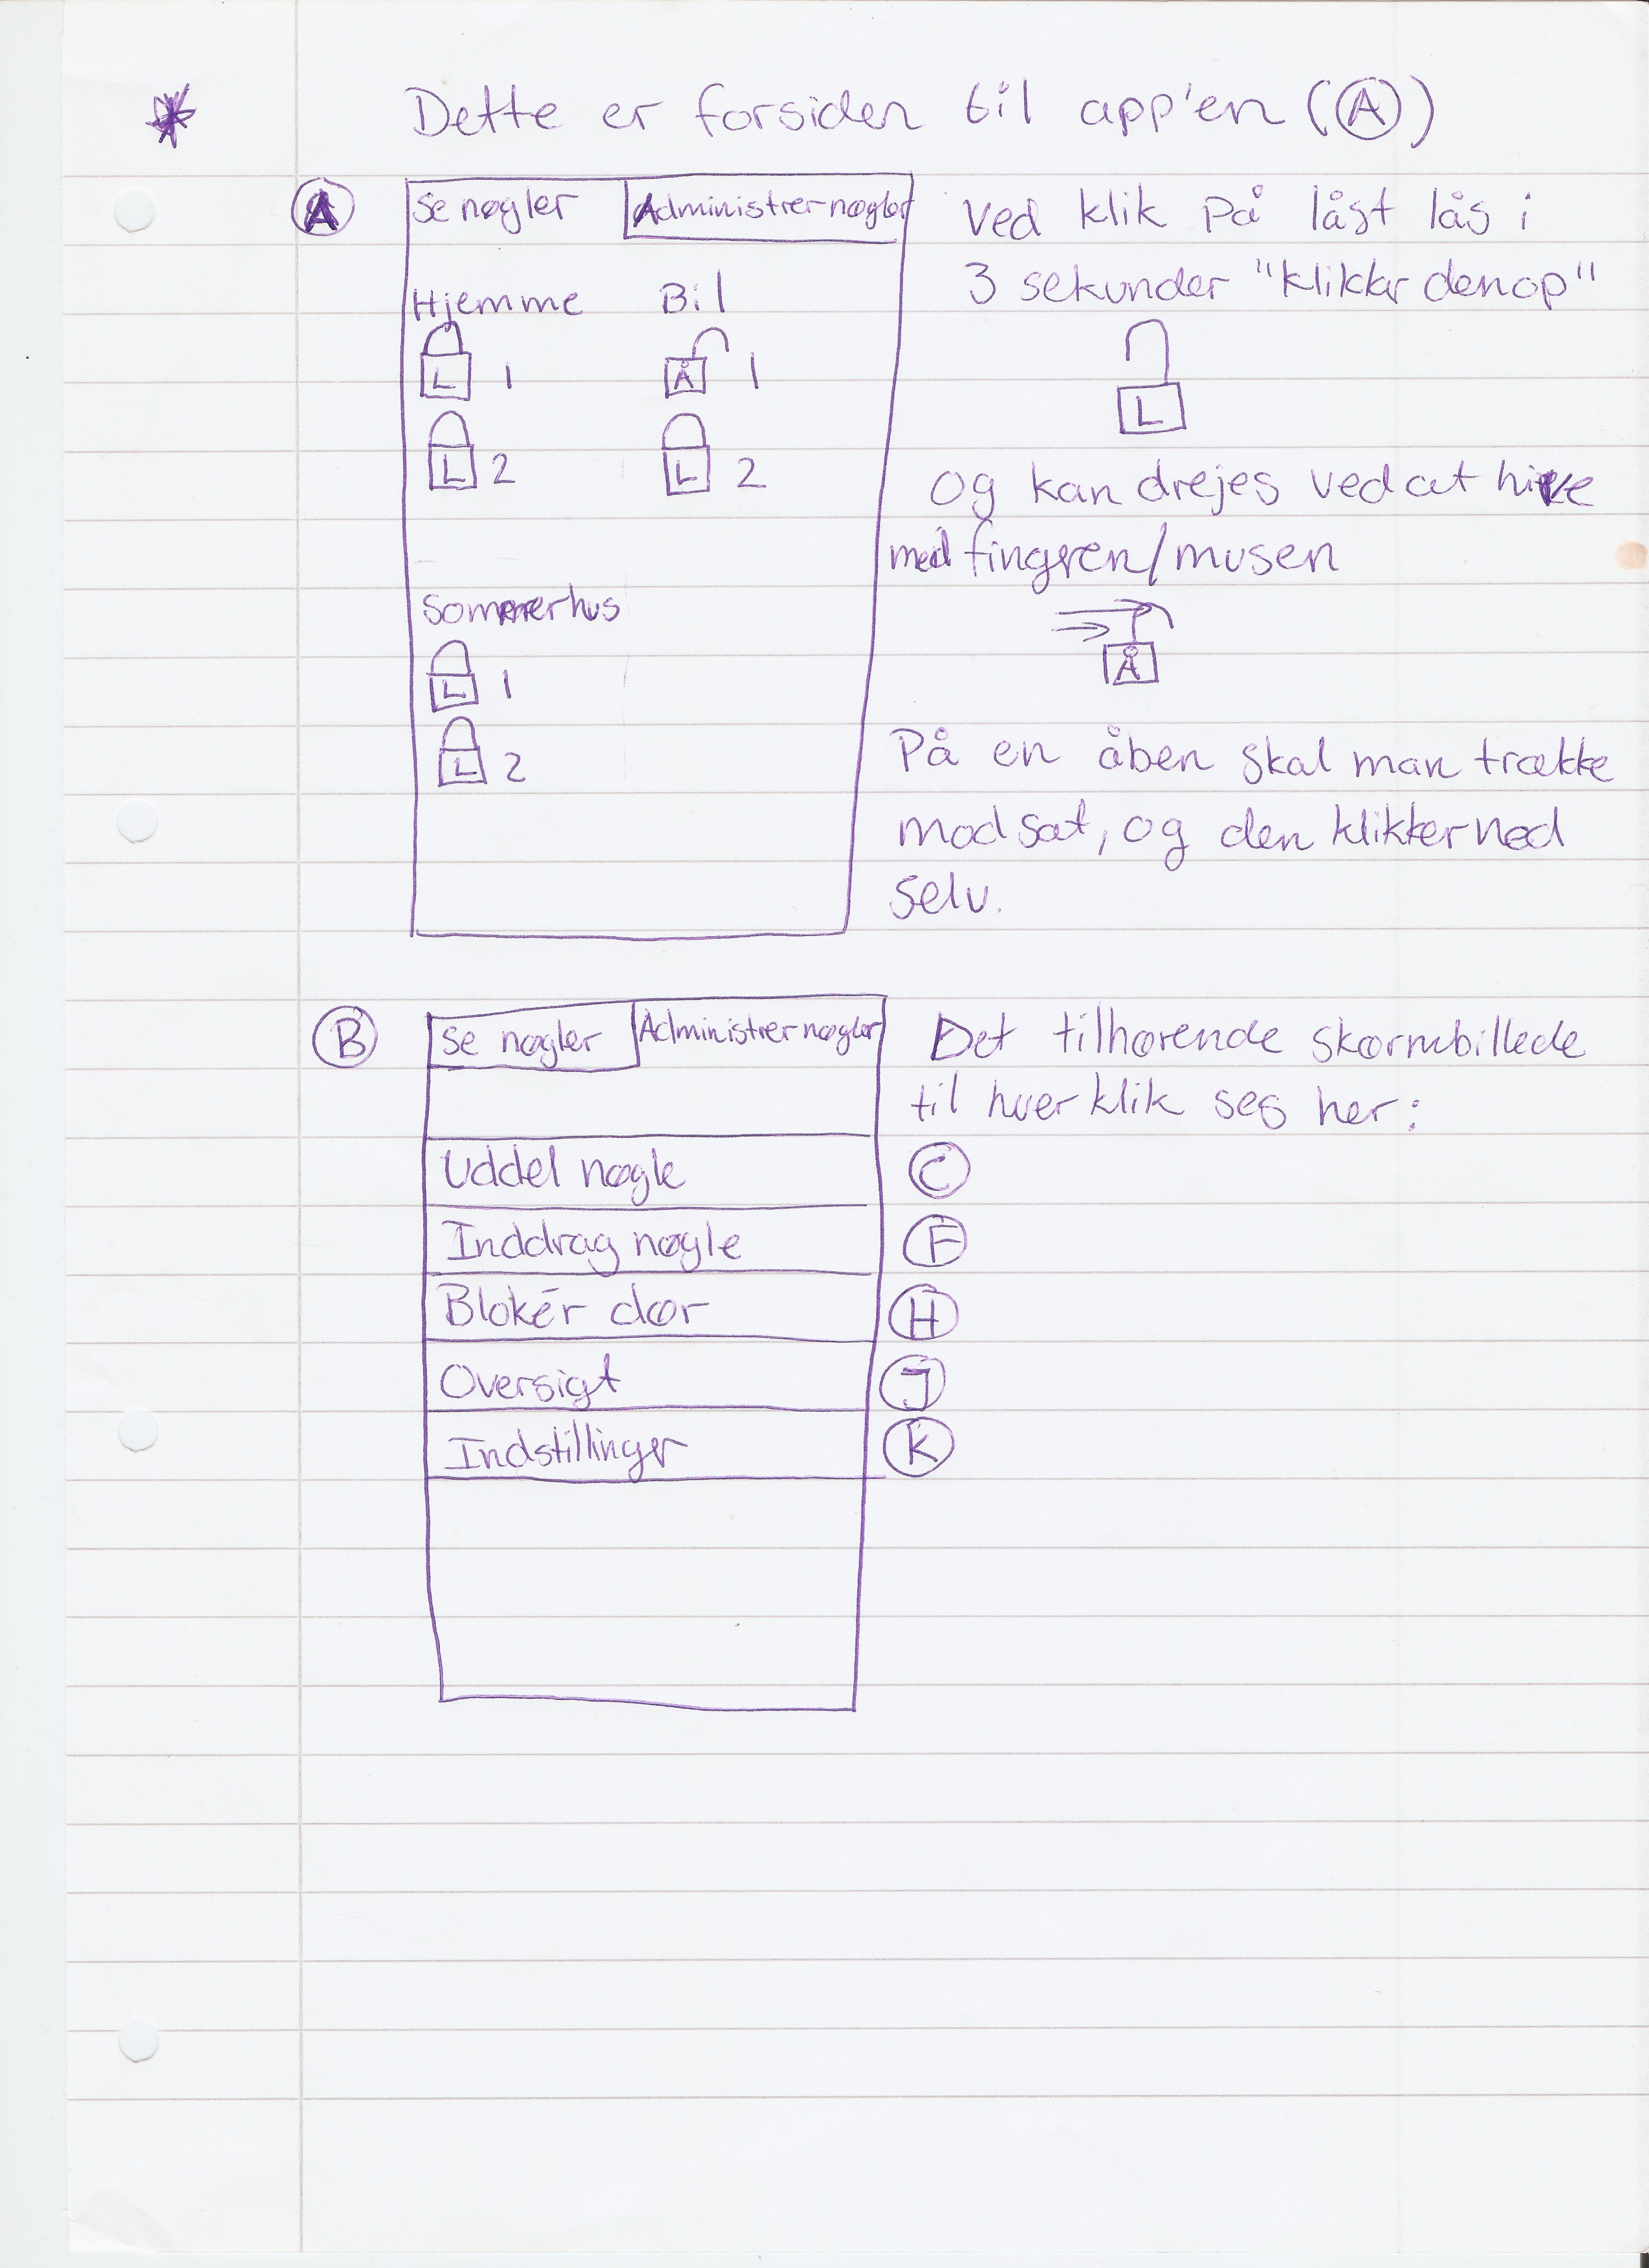
\includegraphics[width=\textwidth]{proto/AB.jpg}
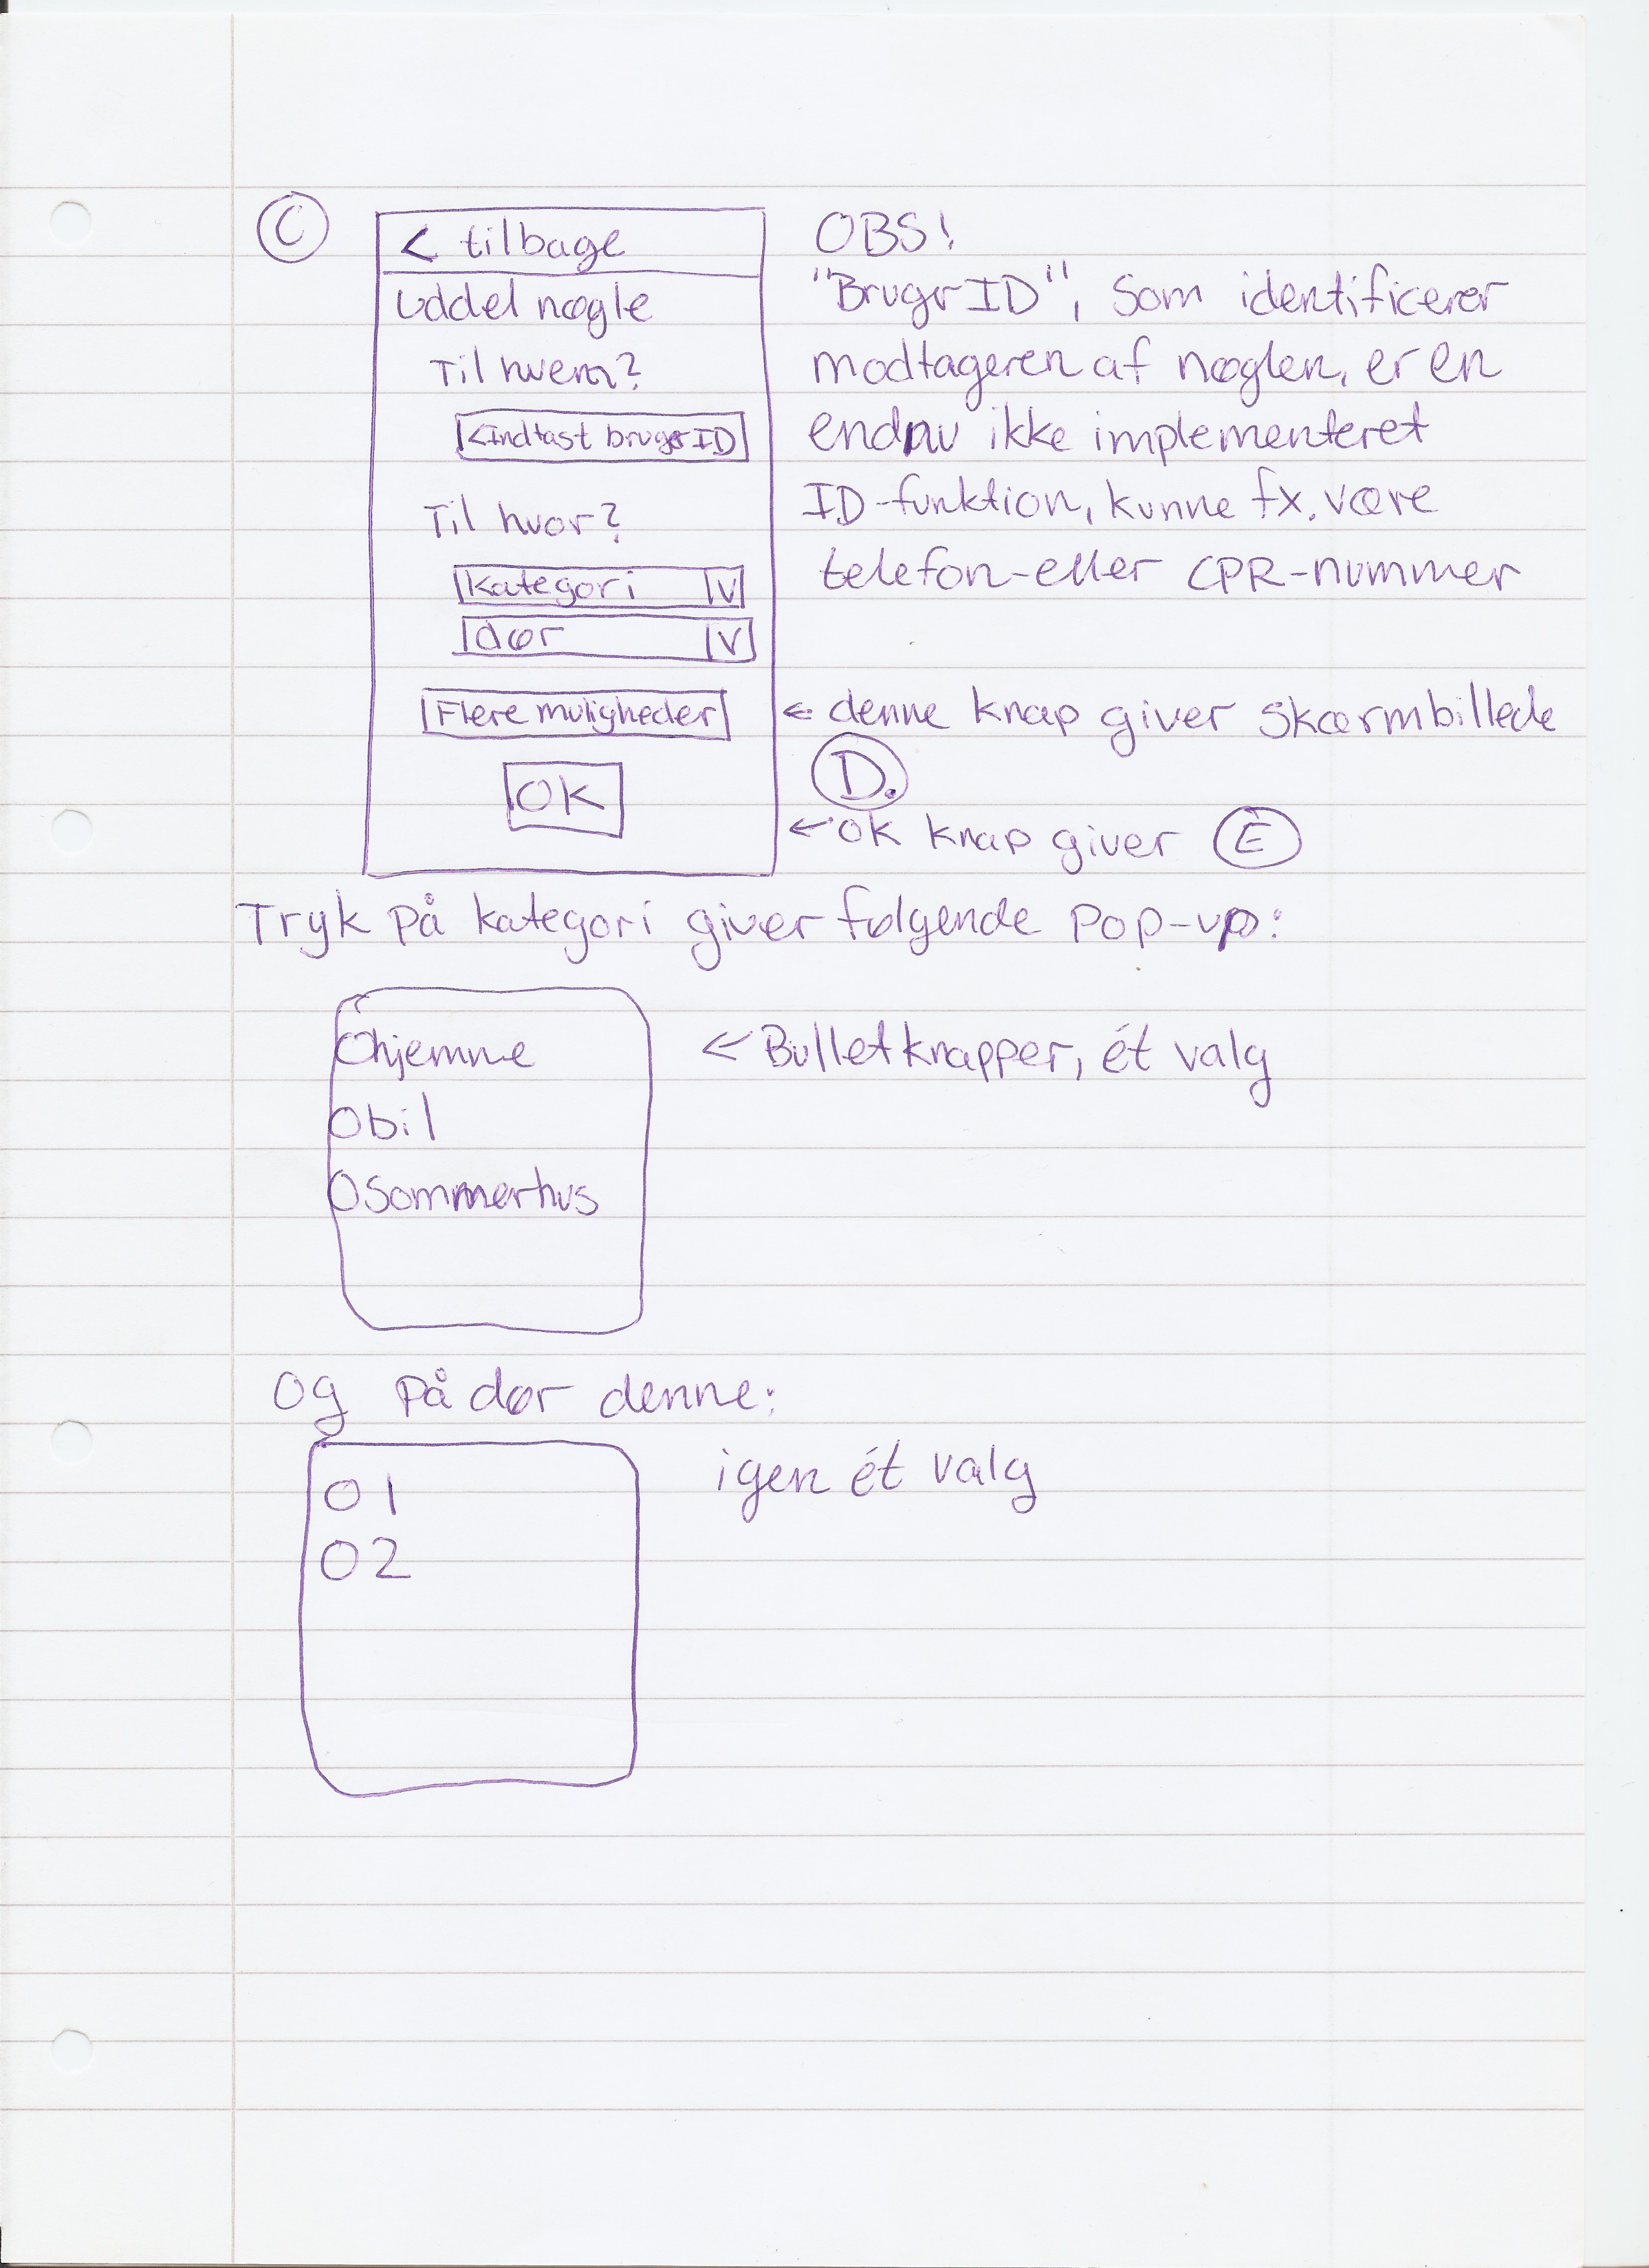
\includegraphics[width=\textwidth]{proto/C.jpg}
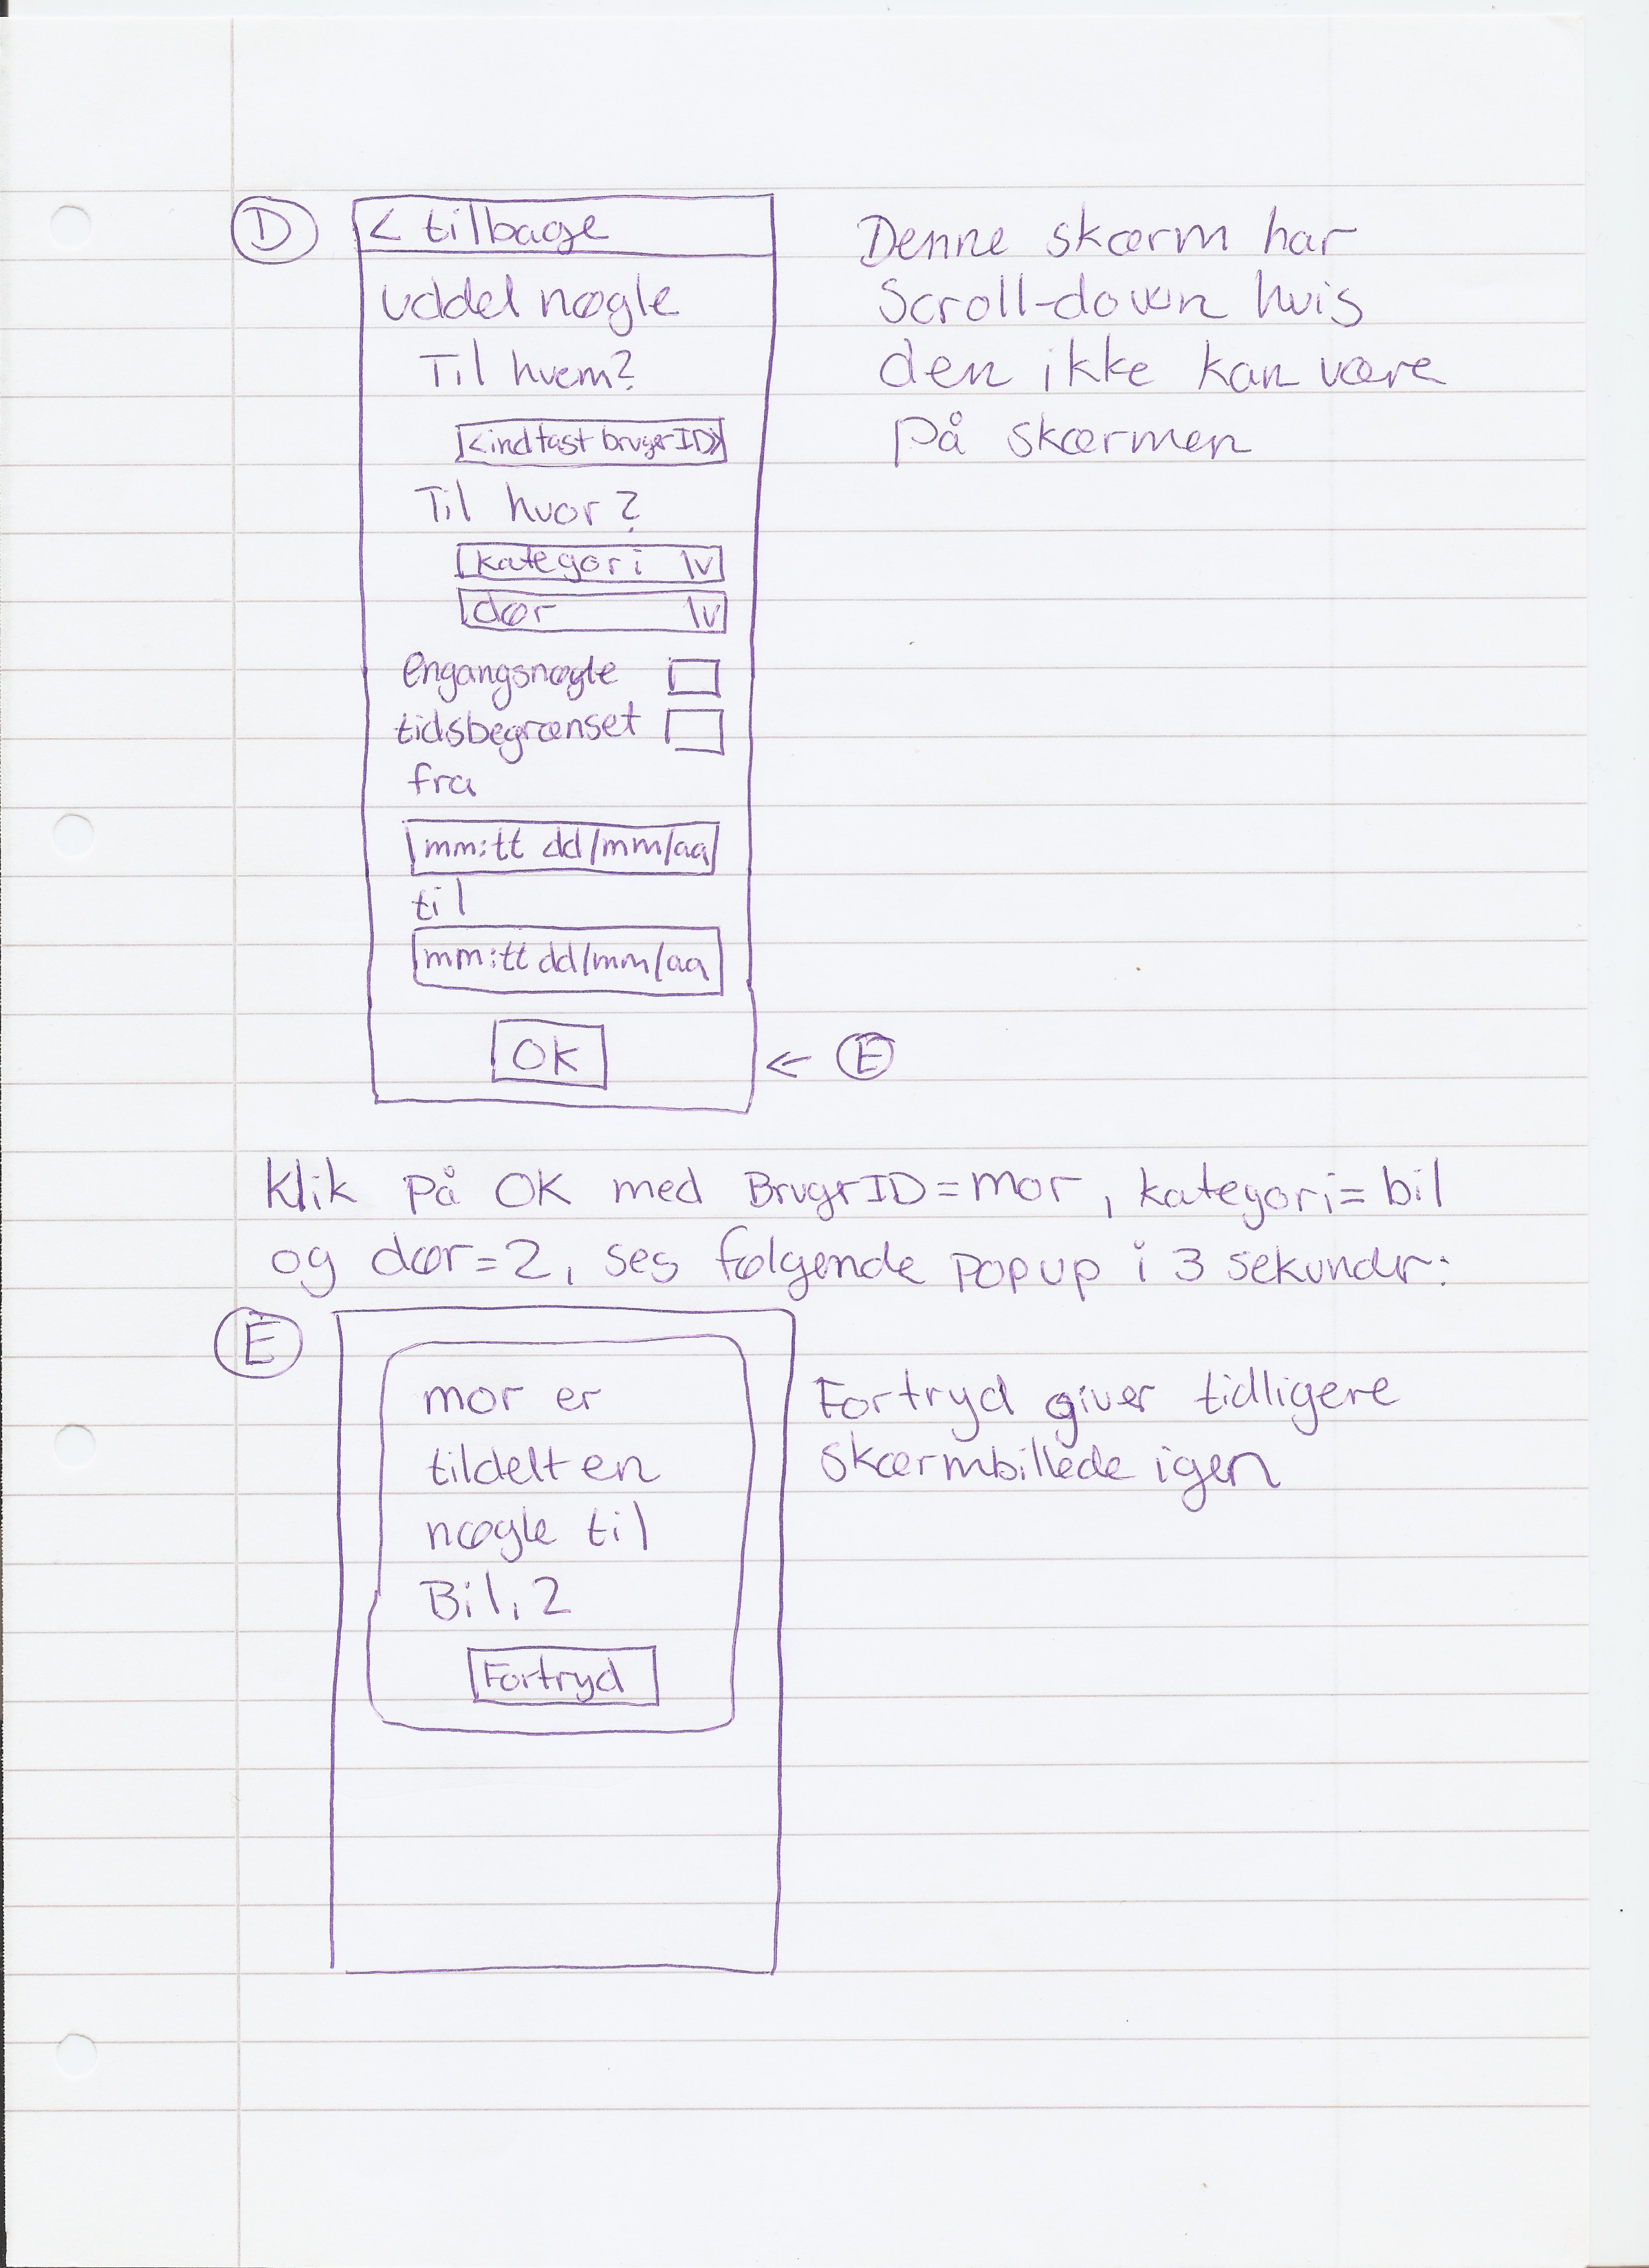
\includegraphics[width=\textwidth]{proto/DE.jpg}
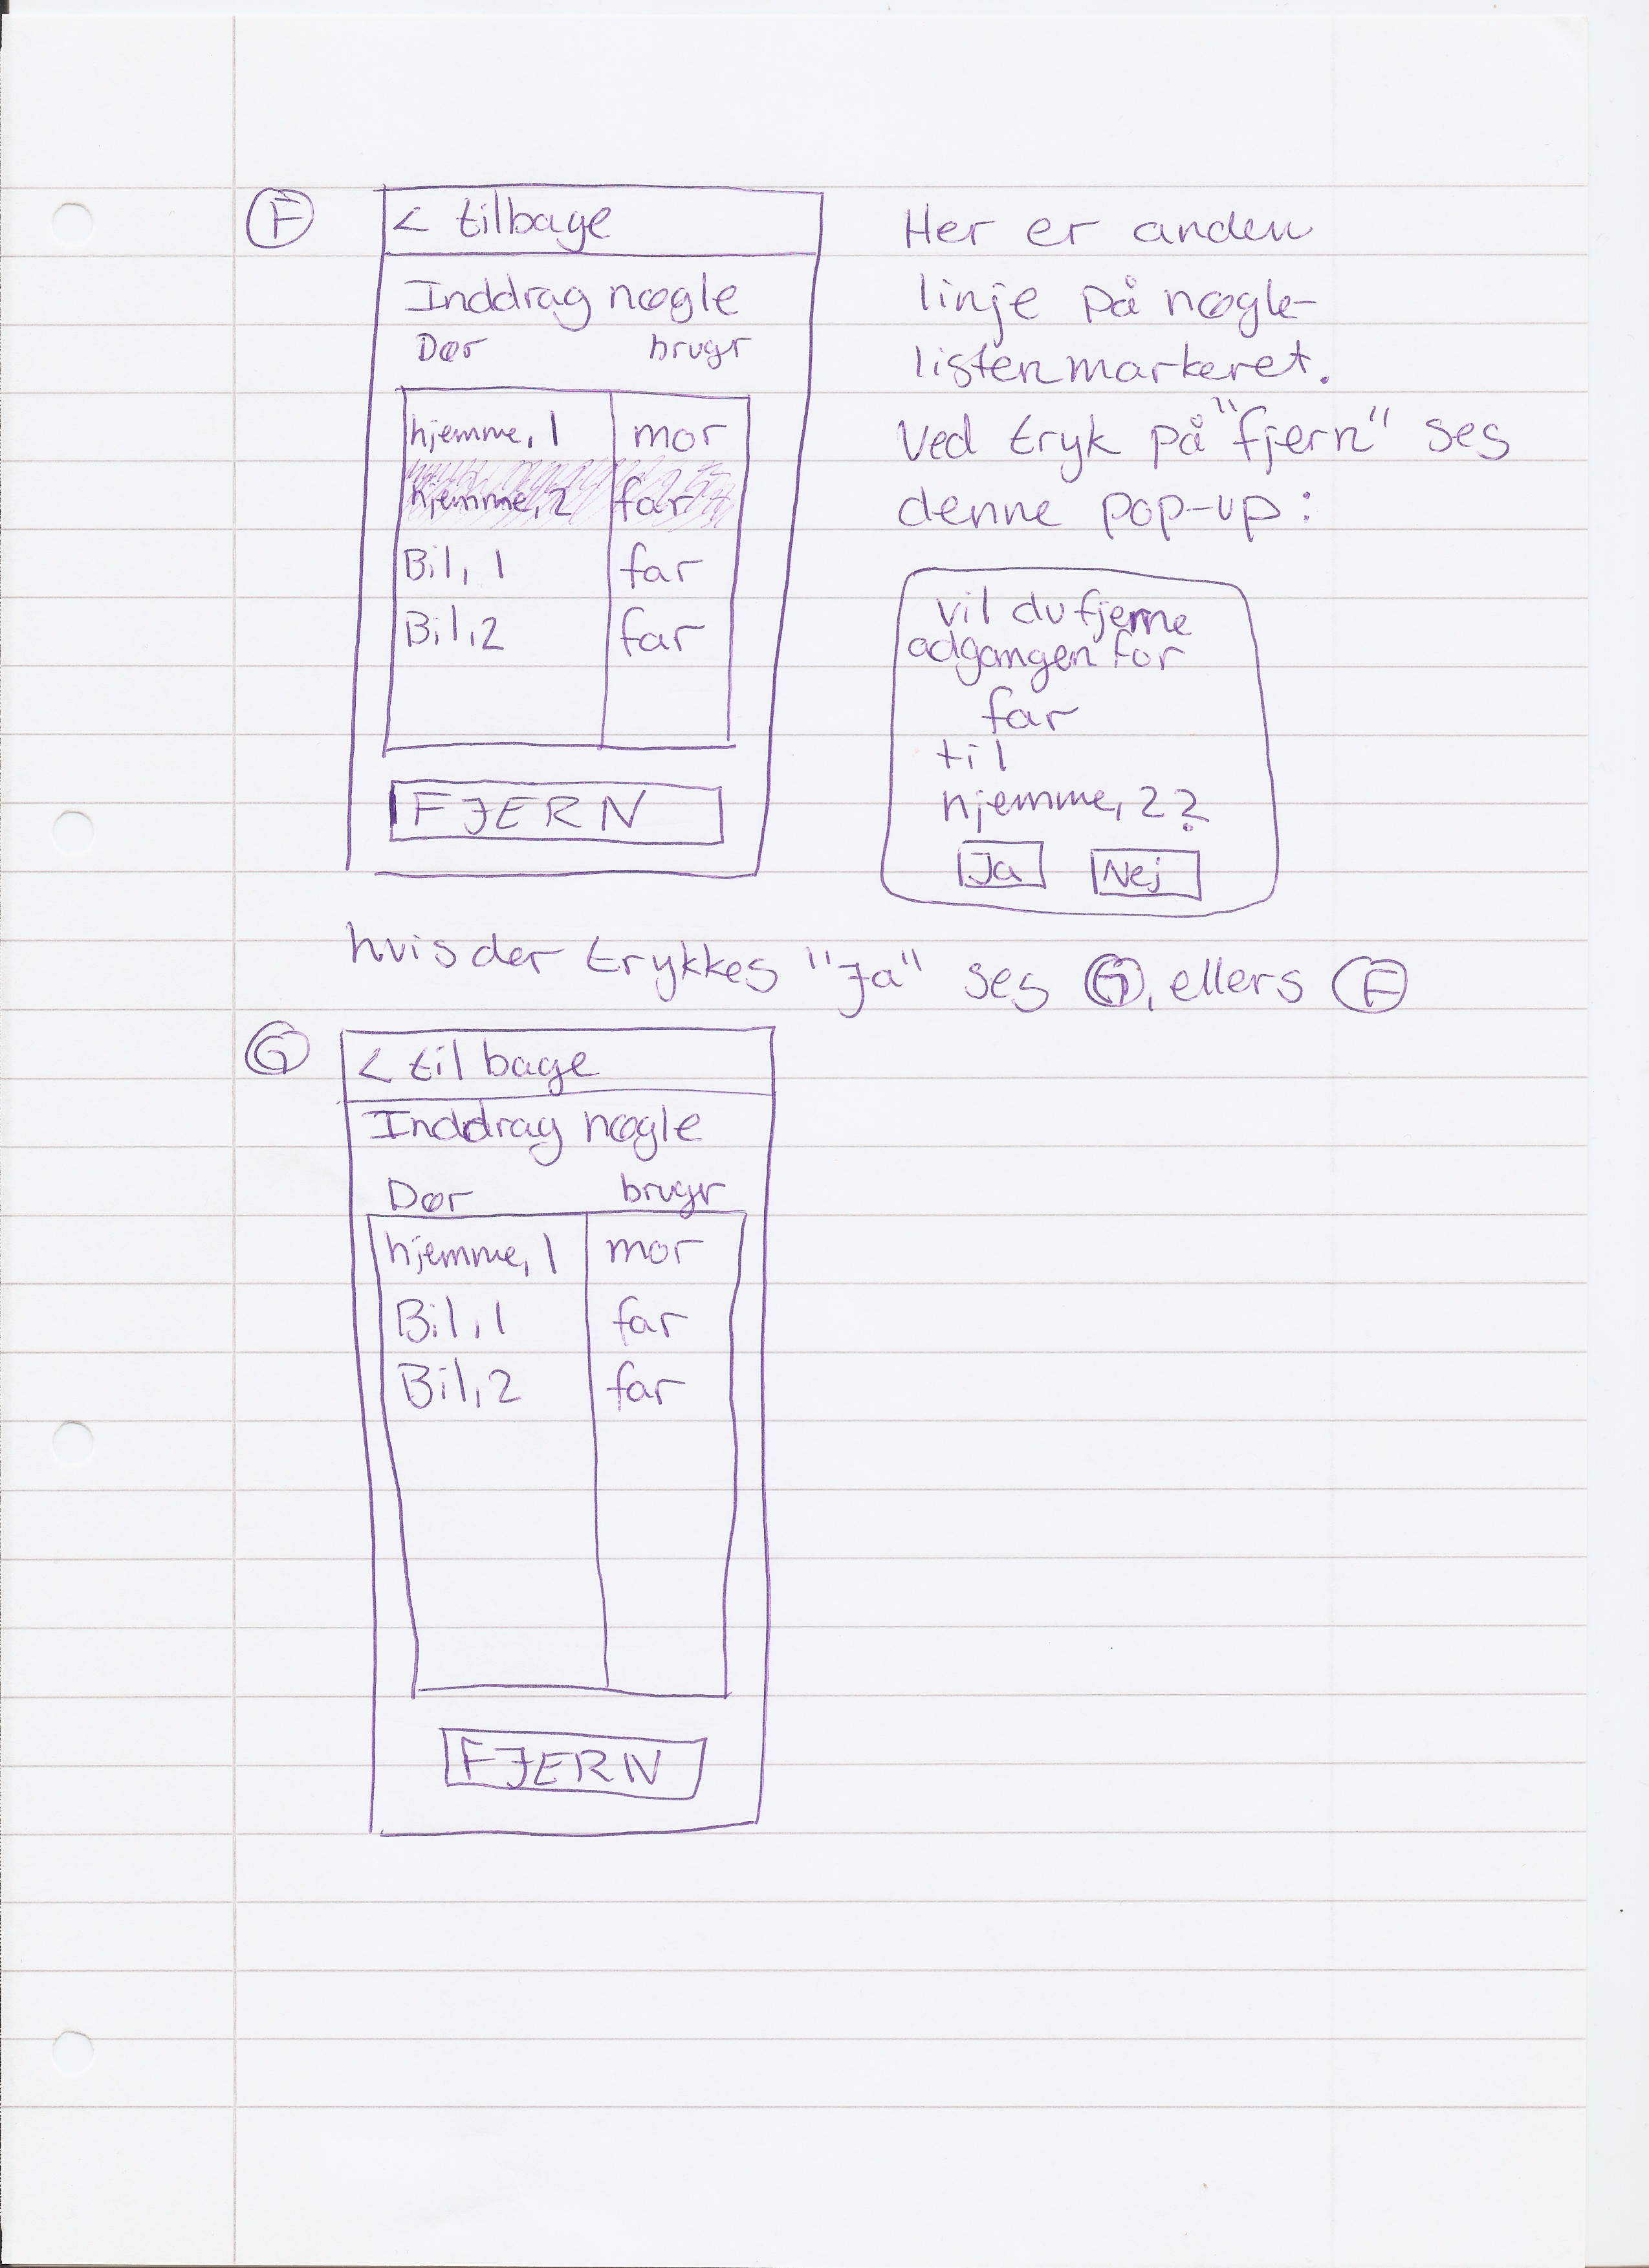
\includegraphics[width=\textwidth]{proto/FG.jpg}
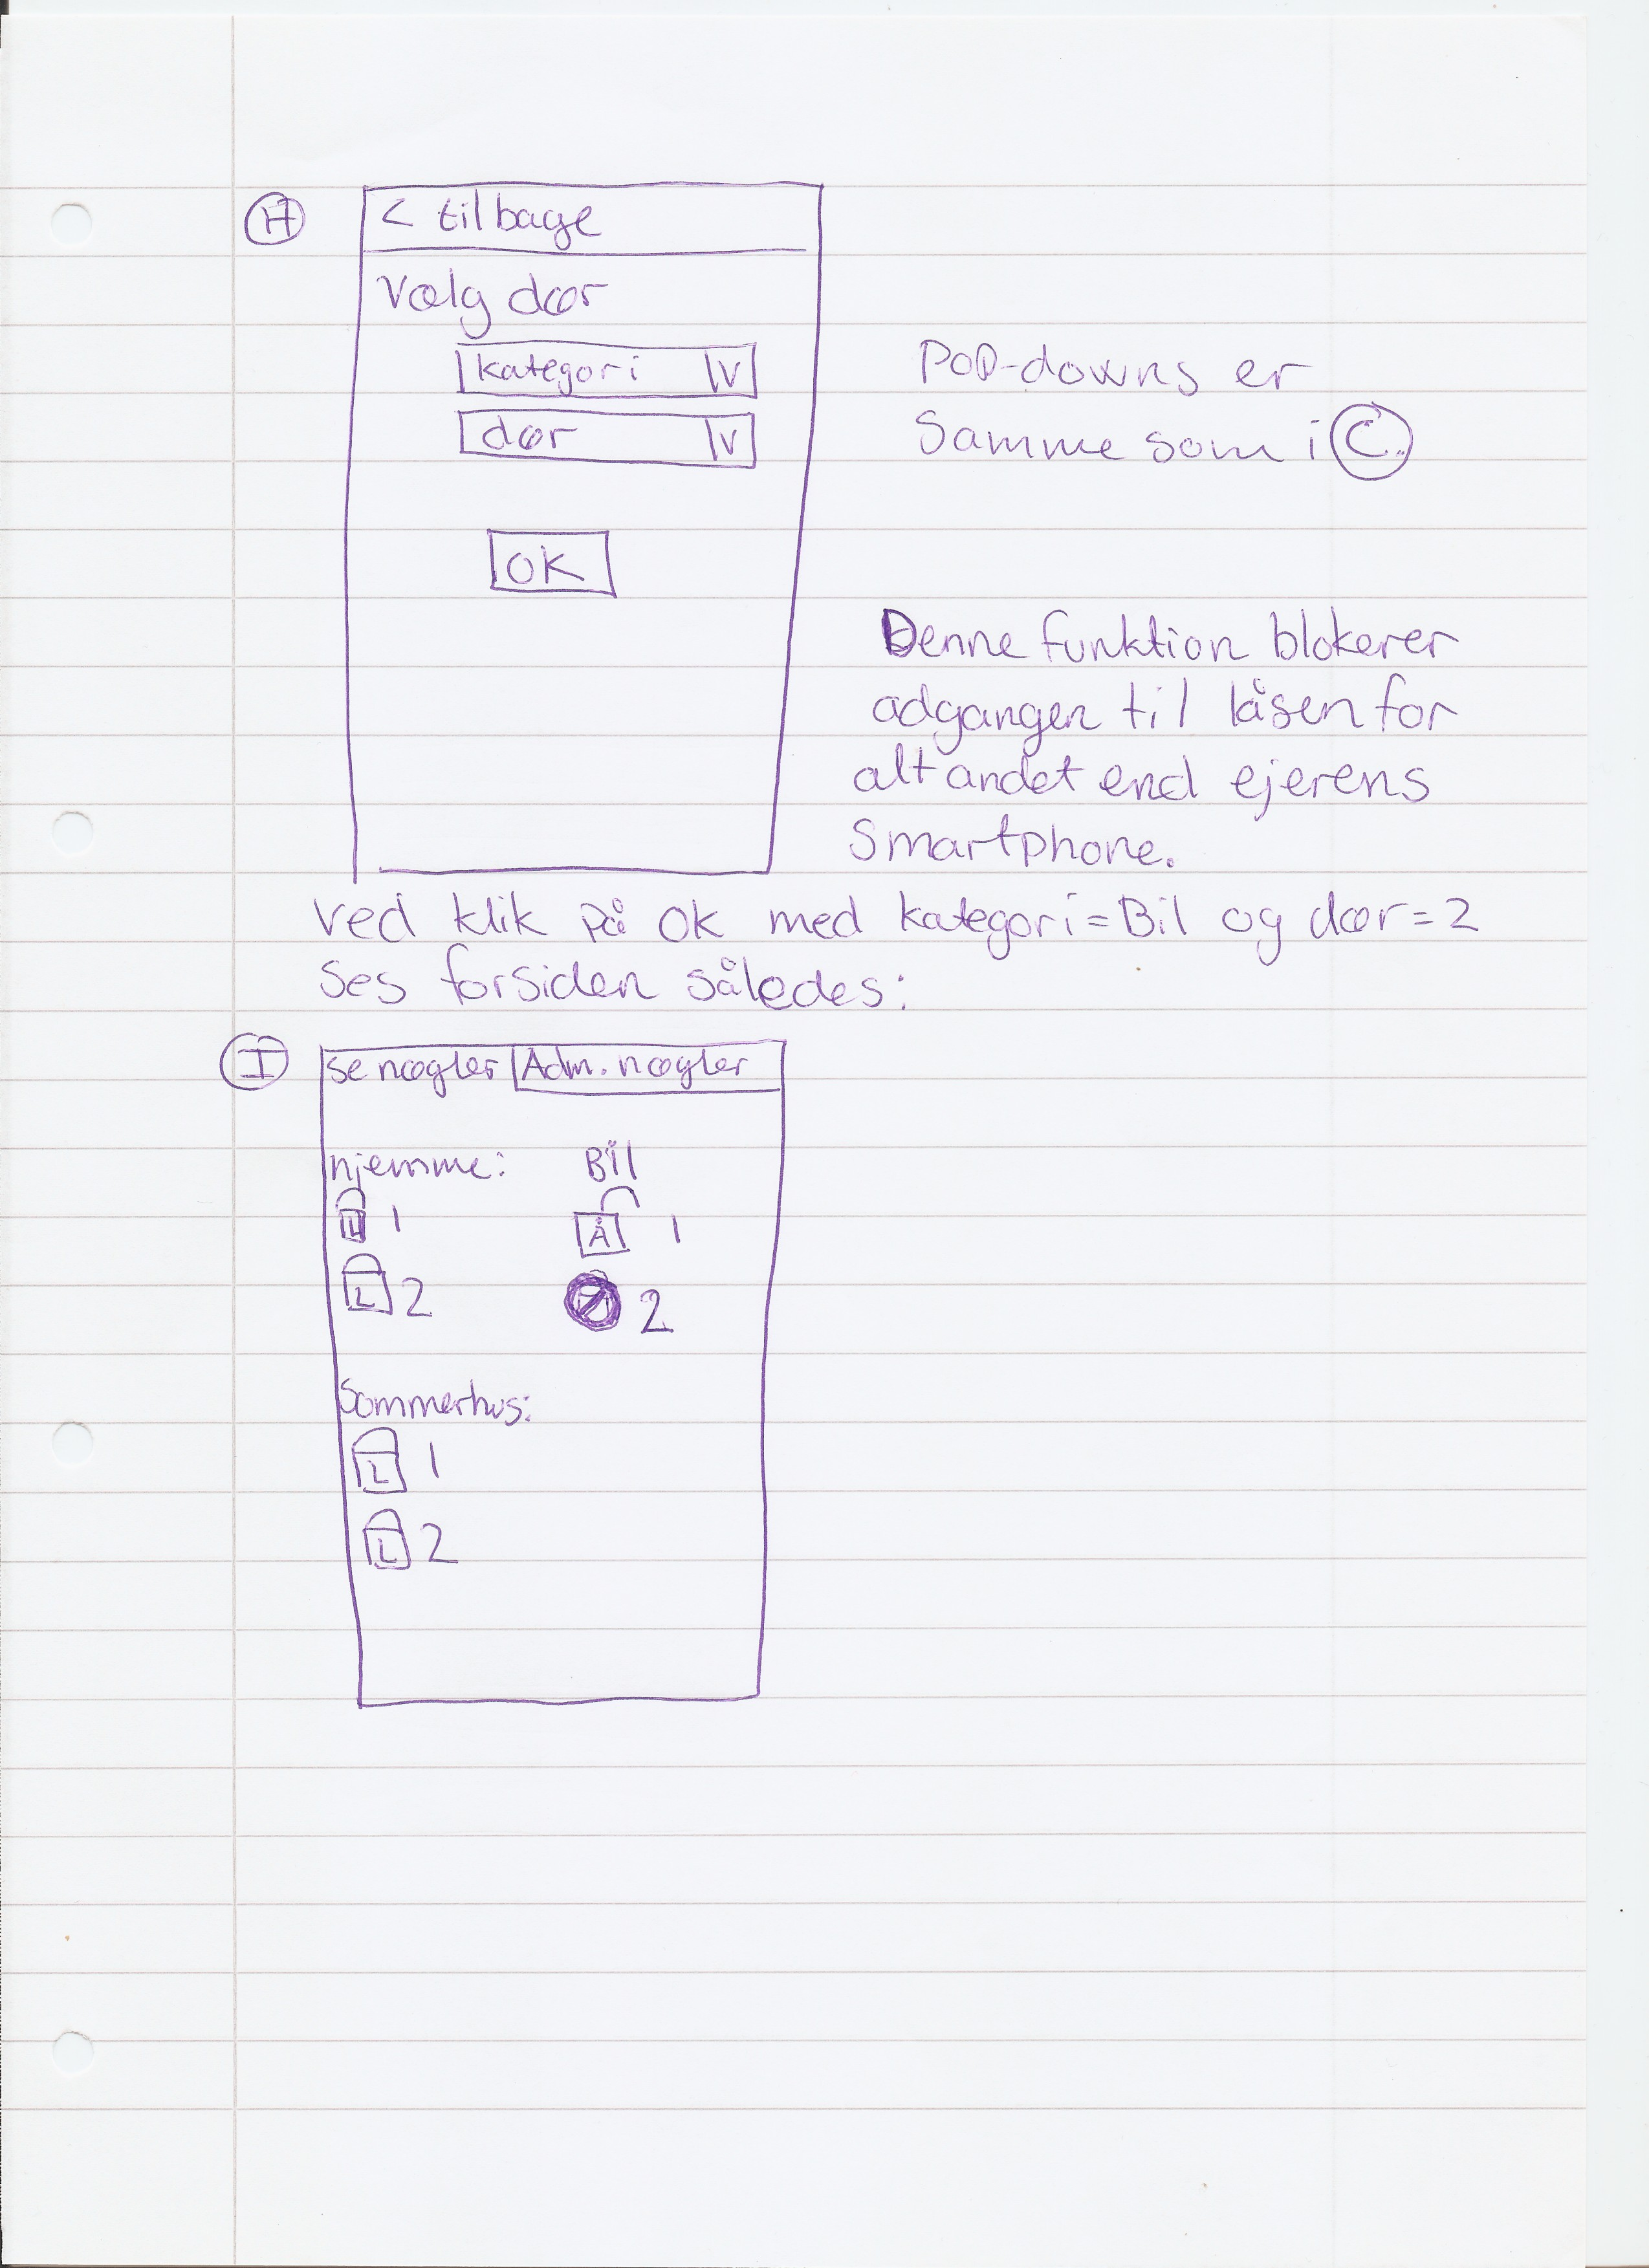
\includegraphics[width=\textwidth]{proto/HI.jpg}
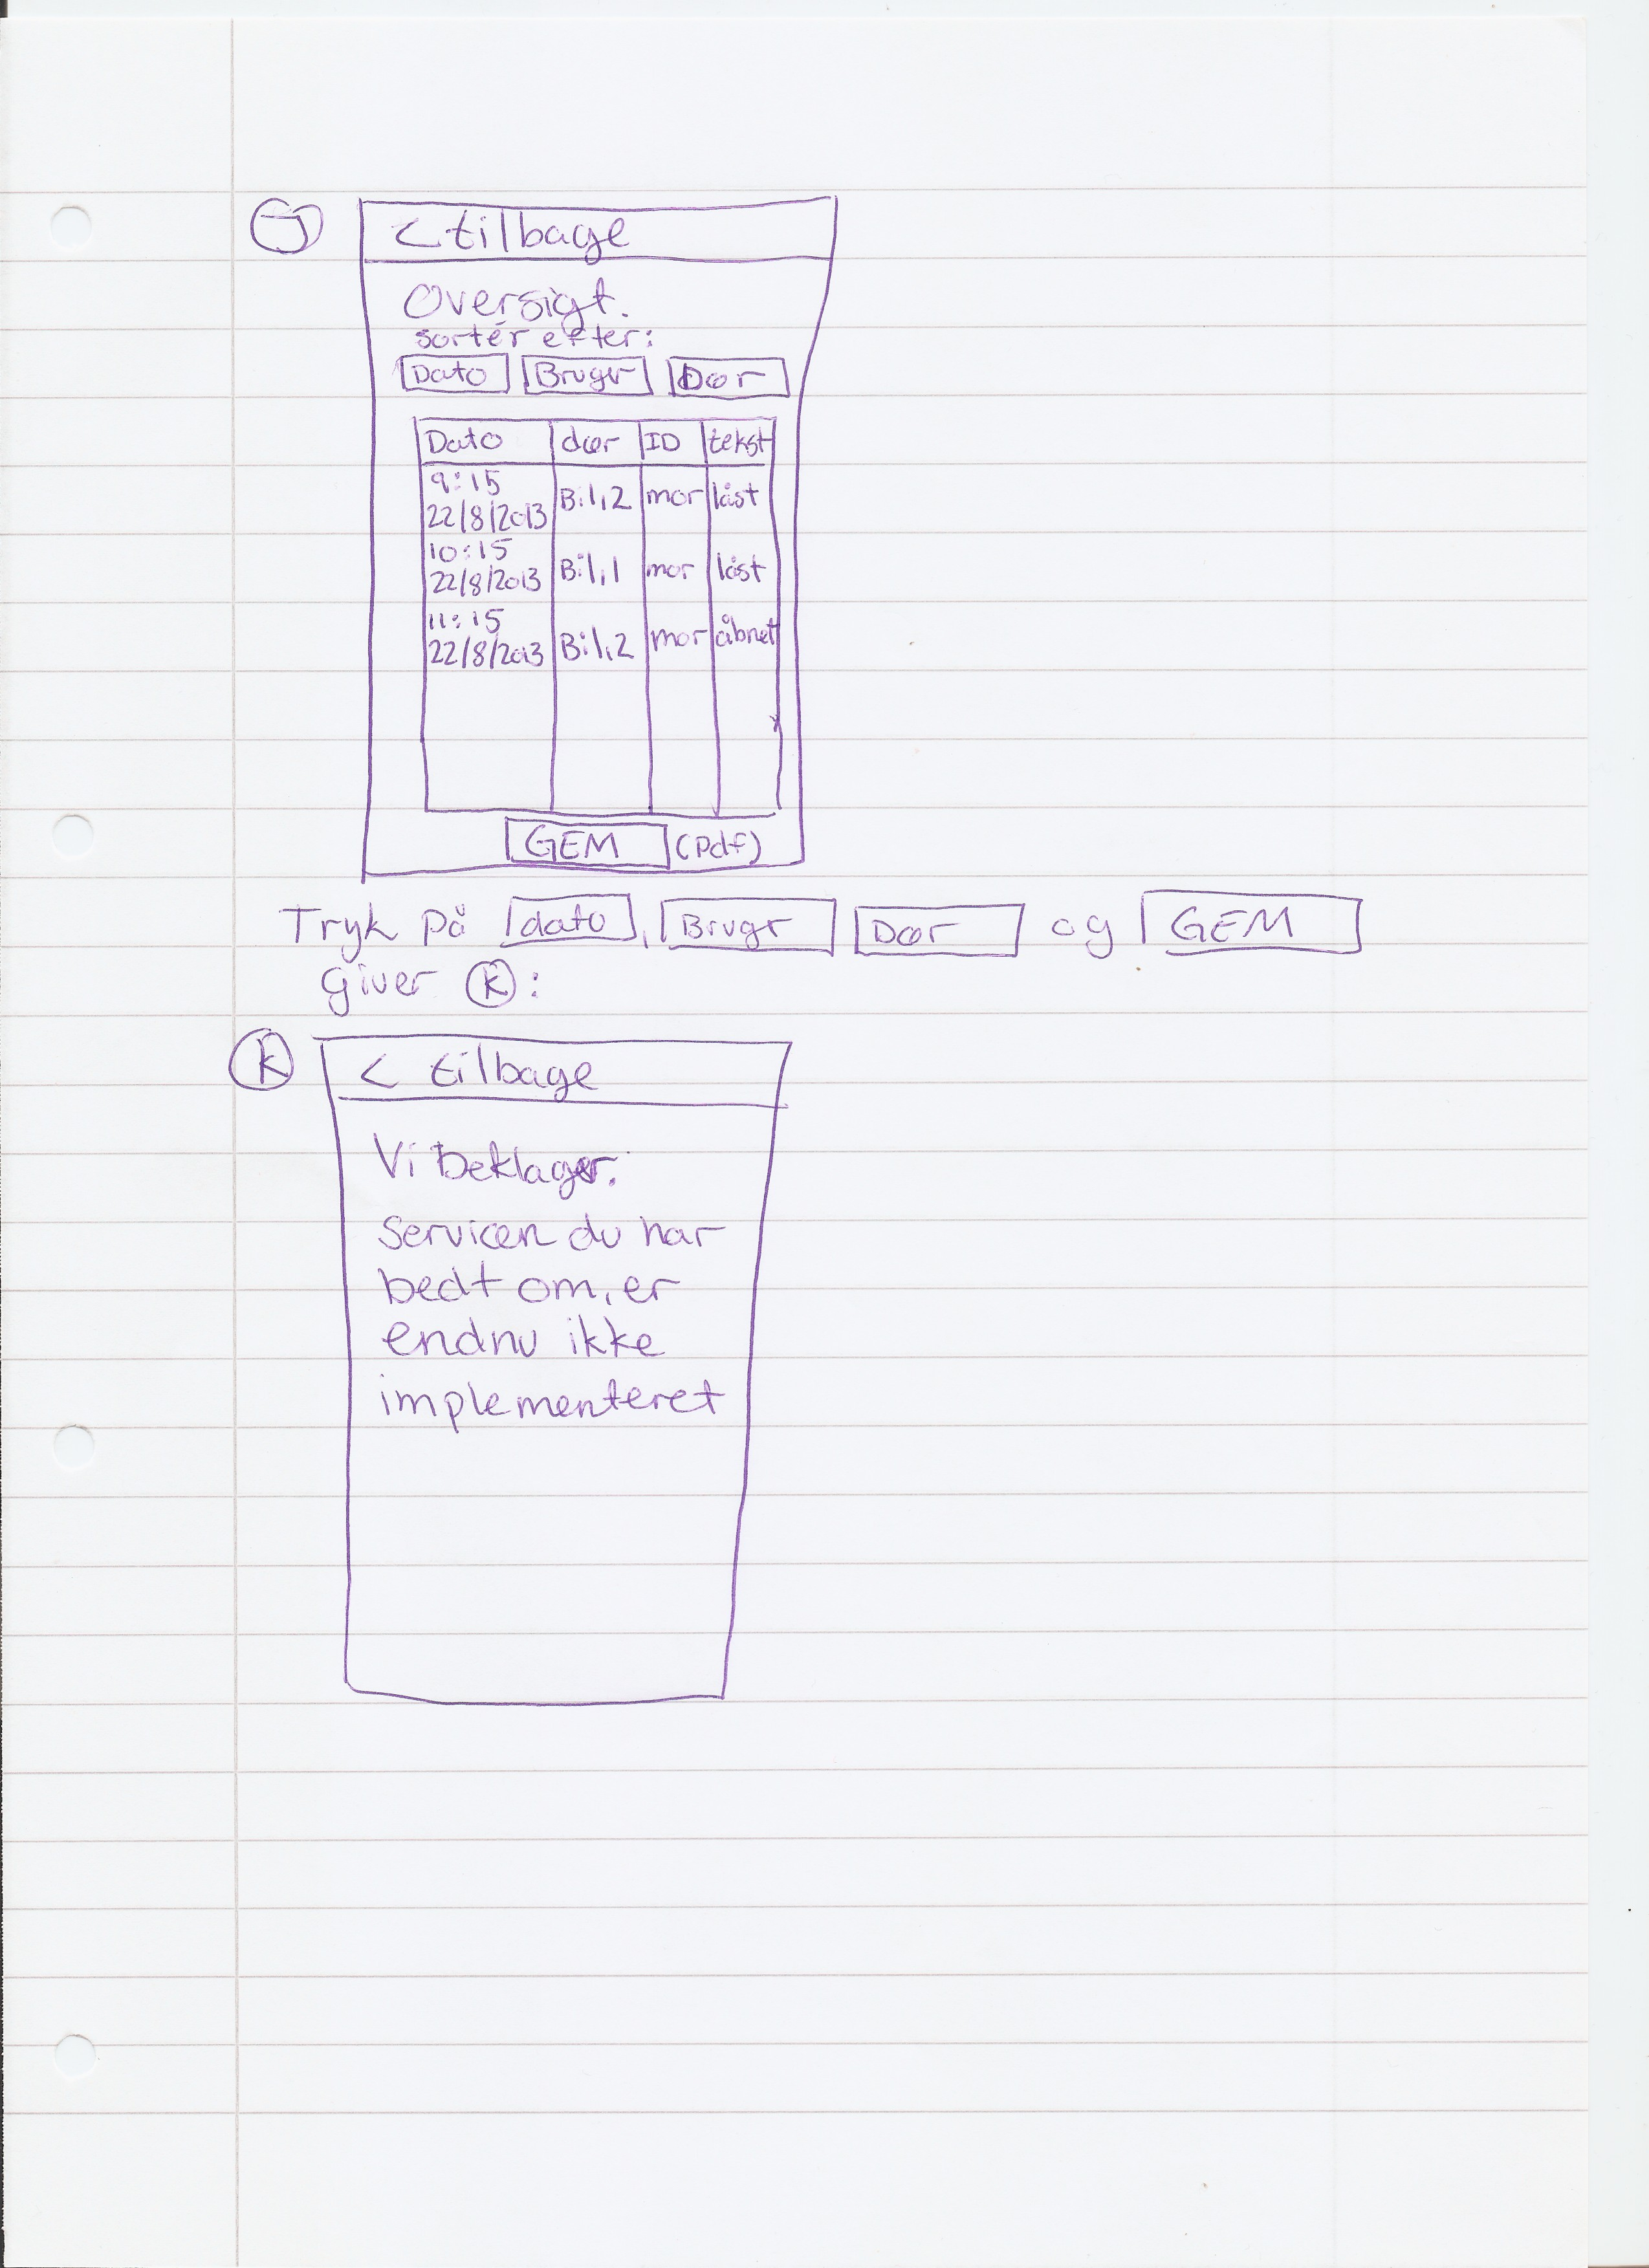
\includegraphics[width=\textwidth]{proto/JK.jpg}

\section{Kommentarer}
\begin{tabular}{|c|c|c|c|c|c|}
	\hline & Forberedelse til interviews & Interviews & Prototype & Rapport & Samlet \\
	\hline Julie & 5 & 3 & 4 & 10 & 22 \\
	\hline Yaser & 6 & 2 & 2 & 14 & 24 \\
	\hline
\end{tabular}

\end{document}